\documentclass[17pt,fancychapters]{report}
\usepackage[a4paper, total={6in, 8in}]{geometry}
\usepackage{listings}
\usepackage{color}
\usepackage{setspace}
\usepackage{fouriernc}
\usepackage{hyperref}
\usepackage{amsfonts}
\usepackage{amsmath}
\usepackage{amsthm}
\usepackage{graphicx}
\usepackage{geometry}
\usepackage{subcaption}
\usepackage{cancel}
\usepackage{tikz}
\usepackage{color}
\usepackage{titlesec}
\usepackage{hyperref}
\usepackage{scalerel}



\titleformat{\chapter}
{\normalfont\LARGE\bfseries}{บทที่ \thechapter}{1em}{}

\titleformat{\section}
{\large\bfseries}{\thesection}{1em}{}

\titleformat{\subsection}
{\normalfont\bfseries}{\thesubsection}{1em}{}

\renewcommand{\figurename}{ภาพที่ }
\renewcommand{\contentsname}{สารบัญ }

\usepackage{fontspec}
\usepackage{xltxtra}
\XeTeXlinebreaklocale "th_TH"
\XeTeXlinebreakskip = 0pt plus 1pt  
\usepackage{fonts-tlwg}

\defaultfontfeatures{Scale=1.6}



\setmainfont[
BoldFont={THSarabunNewBold.ttf},
ItalicFont={THSarabunNewItalic.ttf},
BoldItalicFont={THSarabunNewBoldItalic.ttf}
]{THSarabunNew.ttf}

\linespread{1.3}

\usetikzlibrary{calc,trees,positioning,arrows,chains,shapes.geometric,%
    decorations.pathreplacing,decorations.pathmorphing,shapes,%
    matrix,shapes.symbols}

\geometry{top=1.3in,bottom=1.3in}
\hypersetup{
    colorlinks,
    citecolor=black,
    filecolor=black,
    linkcolor=black,
    urlcolor=black
}

%\SetSymbolFont{letters}{normal}{T1}{cmr}{m}{sl}
%\SetSymbolFont{letters}{bold}  {T1}{cmr}{b}{sl}

\definecolor{DarkerGreen}{RGB}{0,179,45}

\definecolor{Code}{rgb}{0,0,0}
\definecolor{Decorators}{rgb}{0.5,0.5,0.5}
\definecolor{Numbers}{rgb}{0.5,0,0}
\definecolor{MatchingBrackets}{rgb}{0.25,0.5,0.5}
\definecolor{Keywords}{rgb}{0,0,1}
\definecolor{self}{rgb}{0,0,0}
\definecolor{Strings}{rgb}{0,0.63,0}
\definecolor{Comments}{rgb}{0,0.63,1}
\definecolor{Backquotes}{rgb}{0,0,0}
\definecolor{Classname}{rgb}{0,0,0}
\definecolor{FunctionName}{rgb}{0,0,.7}
\definecolor{Operators}{rgb}{0,0,0}
\definecolor{Background}{rgb}{0.98,0.98,0.98}

\lstdefinestyle{python}{
  numbers=left,
  numberstyle=\footnotesize,
  numbersep=1em,
  xleftmargin=1em,
  framextopmargin=2em,
  framexbottommargin=2em,
  showspaces=false,
  showtabs=false,
  showstringspaces=false,
  frame=l,
  tabsize=4,
  % Basic
  basicstyle=\ttfamily\small\setstretch{1},
  backgroundcolor=\color{Background},
  language=Python,
  % Comments
  commentstyle=\color{Comments}\slshape,
  % Strings
  stringstyle=\color{Strings},
  morecomment=[s][\color{Strings}]{"""}{"""},
  morecomment=[s][\color{Strings}]{'''}{'''},
  % keywords
  morekeywords={import,from,class,def,for,while,if,is,in,elif,else,not,and,or,print,break,continue,return,True,False,None,access,as,,del,except,exec,finally,global,import,lambda,pass,print,raise,try,assert},
  keywordstyle={\color{Keywords}\bfseries},
  % additional keywords
  morekeywords={[2]@invariant},
  keywordstyle={[2]\color{Decorators}\slshape},
  emph={self},
  emphstyle={\color{self}\slshape},
  breaklines=true
}

\newtheorem{exmp}{Example}[section]

\newcommand{\codeExample}[2]{
	\begin{exmp}
      #1
      \noindent\begin{minipage}{\linewidth}
      \begin{lstlisting}[style=python]
          #2
      \end{lstlisting}
      \end{minipage}
    \end{exmp}
}

\newcommand\MyLBrace[2]{%
  \left.\rule{0pt}{#1}\right\}\text{#2}}

\newcommand{\myeq}[1]{
  \scalebox{1.1}{$ #1 $}
}  

\tikzset{
>=stealth',
  punktchain/.style={
    rectangle, 
    rounded corners, 
    % fill=black!10,
    draw=black, very thick,
    text width=10em, 
    minimum height=3em, 
    text centered, 
    on chain},
  line/.style={draw, thick, <-},
  element/.style={
    tape,
    top color=white,
    bottom color=blue!50!black!60!,
    minimum width=8em,
    draw=blue!40!black!90, very thick,
    text width=10em, 
    minimum height=3.5em, 
    text centered, 
    on chain},
  every join/.style={->, thick,shorten >=1pt},
  decoration={brace},
  tuborg/.style={decorate},
  tubnode/.style={midway, right=2pt},
}

\title{ระบบแปลภาษาอัตโนมัติด้วยโครงข่ายประสาทเทียม}
\author{พีรเชษฐ  ปอแก้ว}
\date{December 30, 2015}

\begin{document}

\maketitle
\pagenumbering{gobble}
\newpage
\pagenumbering{roman}
\tableofcontents
\newpage
\pagenumbering{arabic}

\chapter[Neural Machine Translation By Jointly Learning to Align and Translate]{Neural Machine Translation By Jointly \\ Learning to Align and Translate}



\begin{flushright}
  Dzmitry Bahdanau, KyungHyun Cho and Yoshua Bengio \\
  {\small แปลโดย พีรเชษฐ ปอแก้ว}
\end{flushright}

\textbf{บทคัดย่อ}

Neural Machine Translation (ระบบแปลภาษาอัตโนมัติด้วยโครงข่ายประสาทเทียม) เป็นวิธีการแปลภาษาอัตโนมัติรูปแบบใหม่ ต่างจากระบบแปลภาษาเชิงสถิติ กล่าวคือ ระบบนี้สามารถปรับจูนพารามิเตอร์ของระบบ (ที่มีเพียงหนึ่งองค์ประกอบ) เพื่อเพิ่มประสิทธิภาพในการแปลได้ ระบบแปลชนิดนีโดยมากอาศัย หลักการของ encoder-decoder ตัว encoder ทำหน้าที่อ่านประโยคต้นทางและบีบอัดให้กลายเป็นเวกเตอร์ที่มีความยาวจำกัด และส่งต่อให้ decoder ทำหน้าที่สร้างประโยคในภาษาปลายทาง ในงานวิจัยนี้เรามีความเห็นว่า การใช้เวกเตอร์ที่มีความยาวจำกัดมาเก็บประโยคทั้งประโยคนั้นเป็นคอขวดของระบบ ที่ทำให้การเพิ่มประสิทธิภาพของการแปลด้วยวิธีนี้ทำได้ยาก เราจึงได้นำเสนอวิธีการใหม่ที่ยอมให้โมเดลสามารถค้นหาส่วนของประโยคที่สัมพันธ์กับคำแปลปัจจุบันได้ โดยไม่จำเป็นต้องผ่านการตัดประโยคออกเป็นส่วนๆ วิธีการนี้ทำให้เราได้ผลลัพธ์ที่ดีเทียบเท่ากับระบบแปลภาษาเชิงสถิติของภาษาอังกฤษเป็นฝรั่งเศส นอกจากนี้ ผลการวิเคราะห์คุณภาพยังแสดงให้เห็นว่า alignment ที่ได้จากระบบนั้นเป็นไปตามสิ่งที่เราคาดหวังไว้ 


\section{บทนำ}
Neural Machine Translation (NMT) เป็นวิธีการแปลภาษาอัตโนมัติรูปแบบใหม่ ซึ่งนำเสนอโดย Kalchbrenner and Blunsom (2013), Sutskever et al. (2014) and Cho et al. (2014b). วิธีการนี้แตกต่างจากระบบแปลภาษาเชิงสถิติ (ดูตัวอย่างเช่น Koehn et al., 2003) ที่จำเป็นต้องสร้างส่วนประกอบย่อยๆ ขึ้นมาแล้วจึงปรับพารามิเตอร์รวมเข้าด้วยกัน วิธีการของ NMT นั้นพยายามสร้างและฝึกสอนระบบโครงข่ายประสาทเทียมที่ต่อกันเป็นระบบเดียว เพื่ออ่านประโยคและแปลเป็นประโยคที่ถูกต้อง

ระบบแปลภาษาด้วยโครงข่ายประสาทเทียมโดยมากนั้นถูกจัดอยู่ในตระกูลของ encoder-decoder  (Sutskever et al., 2014; Cho et al., 2014a) ซึ่งทำหน้าที่จัดการกับภาษาต้นทางและภาษาปลายทางตามลำดับ หรืออาจจะมีส่วนประกอบอื่นเพื่อจัดการกับลักษณะเฉพาะของภาษา หรือการรวมกันของผลลัพธ์ (Hermann and Blunsom, 2014). ตัว encoder ทำหน้าที่อ่านประโยคต้นทางและบีบอัดให้กลายเป็นเวกเตอร์ที่มีความยาวจำกัด ส่วน decoder ทำหน้าที่สร้างประโยคในภาษาปลายทางจากเวกเตอร์ที่ได้นั้น ทั้ง encoder และ decoder ถูกฝึกสอนด้วยคลังตัวอย่างคู่ประโยคเพื่อให้ความน่าจะเป็นของคำแปลที่ถูกต้องมีค่าสูงสุด

ประสิทธิภาพของตัว encoder-decoder นี้อยู่ที่ตัวโครงข่ายประสาทเทียมที่สามารถเก็บเอาข้อมูลที่สำคัญของประโยคไว้ในตัวมันเอง (ซึ่งเป็นเวกเตอร์ขนาดจำกัด) ซึ่งมีข้อจำกัดที่ว่า เมื่อประโยคต้นทางมีความยาวเพิ่มขึ้น ความสามารถในการจดจำข้อมูลลงในเวกเตอร์ก็จะยิ่งลดลง โดยเฉพาะเมื่อความยาวประโยคที่จะแปลนั้นยาวกว่าประโยคที่ใช้ในการฝึกสอน ในงานวิจัยของ Cho et al. (2014b) แสดงให้เห็นว่าประสิทธิภาพของสถาปัยกรรมแบบ encoder-decoder ลดลงอย่างเห็นได้ชัดเมื่อประโยคนำเข้ามีความยาวเพิ่มขึ้น

เพื่อที่จะจัดการกับปัญหานี้ เราได้นำเสนอส่วนขยายของสถาปัตยกรรม encoder-decoder ซึ่งสามารถเรียนรู้ที่จะจับคู่คำและแปลได้ไปพร้อมๆ กัน แต่ละช่วงเวลาของการสร้างคำแปล ตัวโมเดลจะค้นหาตำแหน่งที่เกี่ยวข้องในประโยคภาษาต้นทาง แล้วสร้างคำแปลจากเวกเตอร์ผลลัพธ์ที่สัมพันธ์กับตำแหน่งที่หามาได้นั้น

คุณสมบัติที่แตกต่างระหว่างระบบที่พัฒนาขึ้นกับสถาปัตยกรรม encoder-decoder นั้นก็คือ ระบบนี้ไม่ได้บีบอัด (หรือเข้ารหัส) ประโยคทั้งหมดลงไปที่เวกเตอร์ตัวเดียว แต่ใช้วิธีการเข้ารหัสประโยคต้นทางให้กลายเป็นลำดับของเวกเตอร์ และให้ระบบเลือกสับเซตย่อยของลำดับเวกเตอร์นี้ขึ้นมาแปล วิธีเช่นนี้ทำให้แบบจำลองเป็นอิสระจากการบีบอัดข้อมูลทั้งประโยคลงไปในเวกเตอร์ เราได้แสดงให้เห็นว่าวิธีการนี้แปลประโยคที่ยาวได้มีประสิทธิภาพกว่าวิธีการแบบเดิม

\section{ภูมิหลัง : Neural Machine Translation : NMT}

จากมุมมองของทฤษฏีความน่าจะเป็น การแปล คือ การหาประโยคในภาษาปลายทาง \scalebox{1.2}{$\mathrm{y}$}  ที่ทำให้ ความน่าจะเป็นแบบมีเงื่อนไข (conditional probability) ของประโยคปลายทาง \scalebox{1.2}{$\mathrm{y}$} เมื่อกำหนดประโยคต้นทางเป็น \scalebox{1.2}{$\mathrm{x}$} กล่าวคือ 
\scalebox{1.2}{ $ \mathrm{argmax}_y p(\mathrm{y}| \mathrm{x}) $ } ในระบบ NMT เราจะปรับพารามิเตอร์ทั้งหมดของระบบเพื่อให้ค่าความน่าจะเป็นนี้สูงสุดโดยใช้คลังข้อมูลตัวอย่างคู่ประโยค (training data) เมื่อระบบเรียนรู้ดีแล้ว เราก็สามารถใช้โมเดลนี้ในการแปลประโยคที่ป้อนให้กับระบบแปลโดยการหาประโยคผลลัพธ์ที่ให้ค่าความน่าจะเป็นแบบมีเงื่อนไขสูงสุดเช่นกัน


เร็วๆ นี้ งานวิจัยหลายฉบับได้นำเสนอการใช้โครงข่ายประสาทเทียมเพื่อเรียนรู้การแปลลักษณะนี้ (ดู see, e.g., Kalchbrenner and Blunsom, 2013; Choet al., 2014a; Sutskeveret al.,2014; Choet al., 2014b; Forcada and ̃Neco, 1997)
 โดยส่วนใหญ่วิธีการลักษณะนี้จะประกอบไปด้วยสองส่วนหลัก ส่วนแรกทำหน้าที่เข้ารหัส (encode) ประโยคในภาษาต้นทาง\scalebox{1.2}{ $ \mathrm{x} $} และส่วนที่สองทำหน้าที่ถอดรหัส (decode) เพื่อแปลออกมาเป็นประโยคในภาษาปลายทาง\scalebox{1.2}{ $ \mathrm{y} $} ตัวอย่างเช่น โครงข่ายประสาทเทียมแบบป้อนกลับ (Recurrent neural network : RNN) ได้ถูกพัฒนาโดย (Choet al., 2014a) และ (Sutskeveret al., 2014) เพื่อเข้ารหัสประโยคที่มีความยาวไม่แน่นอนให้กลายเป็นเวกเตอร์ และถอดรหัส (แปล) มาเป็นประโยคปลายทางที่มีความยาวไม่แน่นอนเช่นกันได้

แม้ว่าวิธีการเช่นนี้จะเป็นวิธีการใหม่ แต่ระบบแปลด้วยโครงข่ายประสาทเทียมได้แสดงให้เห็นถึงผลลัพธ์การแปลที่ดี Sutskeveret al.(2014) ได้รายงานว่าระบบแปลด้วยโครงข่ายประสาทเทียมแบบป้อนกลับที่อาศัยหลักการของ Long short-term memory (LSTM) ได้ให้ค่าความถูกต้องของผลการแปลใกล้เคียงระบบที่เป็นมาตรฐาน (state-of-the-art) ที่อาศัยแบบจำลองเชิงสถิติ ซึ่งทดสอบด้วยคลังข้อมูลประโยคคำแปลจากภาษาอังกฤษเป็นฝรั่งเศส นอกจากนี้การใช้โครงข่ายประสาทเทียมร่วมกับระบบแปลเดิม เช่น การใช้โครงข่ายประสาทเทียมเพื่อคิดคะแนนคู่คำแปลในตารางคำแปล (phrase table) (Choet al., 2014a) หรือใช้ในการเรียงลำดับตัวเลือก (candidate) (Sutskeveret al., 2014) ต่างก็ให้ผลลัพธ์ที่ดีกว่าระบบเดิม

\subsection{RNN Encoder-Decoder}

ในส่วนนี้ จะอธิบายเฟรมเวิร์คของ RNN Encoder-Decoder ที่พัฒนาโดย Cho et al.(2014a) และ Sutskeveret al.(2014) ซึ่งเราพัฒนาวิธีการที่ทำให้ระบบสามารถเลือกคำและแปลได้พร้อมๆ กัน

สถาปัตยกรรมแบบเข้ารหัส-ถอดรหัส (Encoder-Decoder) ตัวเข้ารหัสจะอ่านลำดับของคำในประโยค ซึ่งลำดับนี้ถูกแทนค่าด้วยลำดับของเวกเตอร์ \scalebox{1.1}{$ \mathrm{x} = (x_1, \ldots , x_{T_x}) $}  เพื่อสร้างเวกเตอร์ $ c $ วิธีการทั่วไปที่ใช้นั้นคือใช้ RNN โดยที่
\begin{equation}
\scalebox{1.1}{$ h_t = f(x_t,h_{t-1}) $}
\end{equation}

\noindent และ

\begin{equation}
\scalebox{1.1}{$ c = q(\{h_1,...,h_{T_x}\}), $}
\end{equation}

\noindent โดยที่ \scalebox{1.1}{$ h_t \in \mathbb{R}^n $} คือ hidden state ณ เวลา \scalebox{1.1}{$ t $} และ \scalebox{1.1}{$ c $} คือเวกเตอร์ที่ถูกสร้างจากลำดับของ hidden state ส่วน \scalebox{1.1}{$ f $} และ \scalebox{1.1}{$ q $} เป็นฟังก์ชั่นแบบไม่เชิงเส้น ซึ่งในงานของ Sutskever et al. (2014) นั้นใช้ LSTM สำหรับฟังก์ชั่น f และ กำหนดให้    \scalebox{1.1}{$ q(\{h_1,...,h_{T_x}\}) = h_{T_x}$} 

สำหรับตัวถอดรหัส Decoder นั้นมักจะถูกฝึกสอนให้ทำนายคำถัดไป \myeq{y_t} โดยมีค่าตั้งต้นเป็นเวกเตอร์ \myeq{c} และคำที่ถูกทำนายขึ้นมาก่อนหน้า \myeq{ \{y_1,...,y_{t'-1}\} } ในอีกความหมายหนึ่ง ตัวถอดรหัสนี้เป็นตัวคำนวณค่าความน่าจะเป็นของประโยคปลายทาง \myeq{y} โดยการแยกคำในประโยคออกเป็นส่วนๆ แล้วคำนวณหาความน่าจะเป็น (Joint Probability) แบบเป็นลำดับ


\begin{equation}
  \scaleto{p(y) = \prod_{t=1}^{T} p(y_t | \{y_1,...,y_{t-1}\},c)}{28pt}
\end{equation}

\noindent โดยที่ประโยคปลายทาง \myeq{ y = (y_1,...,y_{T_y}) } เมื่อใช้ RNN แล้วทำให้แต่ละพจน์ของ conditional probability สามารถนิยามได้ดังนี้

\begin{equation}
\myeq{ p(y_t | \{y_t,...,y_{t-1}\},c) = g(y_{t-1},s_t,c), }
\end{equation}

\noindent โดยที่ \myeq{g} เป็นฟังก์ชั่นไม่เชิงเส้น (อาจมีหลายเลเยอร์) ที่มีไว้คำนวณความน่าจะเป็นของคำที่กำลังทำนาย \myeq{y_t} และ \myeq{s_t} คือ hidden state ของ RNN ซึ่งในความเป็นจริงแล้วรูปแบบสถาปัตยกรรมแบบอื่น เช่น การใช้ RNN ร่วมกับ de-convolution neural network ก็สามารถใช้ได้เช่นกัน (Kalchbrenner and Blunsom, 2013)

\section{Learning to Align and Translate}

ในหัวข้อย่อยนี้ เรานำเสนอสถาปัตยกรรมแบบใหม่สำหรับ NMT วิธีการใหม่นี้ประกอบด้วย bidirectional RNN เพื่อใช้เป็น encoder และตัว decoder ที่สามารถค้นหาส่วนของประโยคที่จะแปลระหว่างการสร้างประโยคปลายทางด้วย



\subsection{Decoder: General Description}

ในสถาปัตยกรรมแบบใหม่นี้ เราให้นิยามของ conditional probability ใน Eq. (2) เป็นดังนี้

\begin{equation}
\scalebox{1.1}{$ p(y_i|y_1,...,y_{i-1},x) = g(y_{i-1},s_i,c_i) $}
\end{equation}

\noindent โดยที่ \myeq{ s_i } คือ hidden state ณ เวลา \myeq{i} ซึ่งถูกคำนวณโดย

\begin{equation}
\myeq{s_i = f(s_{i-1},y_{i-1},c_i)}
\end{equation}

ซึ่งแตกต่างจากระบบ encoder-decoder เดิมที่ตัว context vector  \myeq{c} นี้จะเปลี่ยนไปทุกๆ ช่วงเวลา \myeq{i} สำหรับการทำนายคำแปล \myeq{ y_i }

Context vector \myeq{ c_i} นี้ถูกคำนวณจากลำดับของ annotations \myeq{ (h1,...,h_{t_x}) }ซึ่งเป็นตัวแทนของประโยคอินพุต แต่ละ\myeq{ h_i} นั้นเก็บข้อมูลทั้งประโยคแต่ให้น้ำหนักไปที่บริบทรอบๆ คำที่\myeq{i}ของอินพุต เราจะอธิบายถึงวิธีการหา annotations นี้ในหัวข้อย่อยถัดไป

ตัว Context vector \myeq{c_i} นี้ถูกคำนวนโดยค่าเฉลี่ยถ่วงน้ำหนักของ annotations \myeq{h_i}

\begin{equation}
  \scaleto{c_i = \sum_{j=1}^{T_x}\alpha_{ij}h_j}{28pt}
\end{equation}


\noindent โดยที่ \myeq{\alpha_{ij}} คือ น้ำหนักที่ให้กับ annotatation\myeq{h_j} ณ ช่วงเวลา\myeq{i} ที่คำนวณโดย

\begin{equation}
  \scaleto{\alpha_{ij} = \frac{\mathrm{exp}(e_ij)}{\sum_{k=1}^{T_x}\mathrm{exp}(e_{ik})}}{28pt}
\end{equation}


\noindent โดยที่
\begin{equation}
  \myeq{e_{ij} = a(s_{i-1},h_j)}
\end{equation}

เรียกว่าเป็น alignment model ที่ให้คะแนนความสัมพันธ์ระหว่างคำ รอบๆ ตำแหน่ง \myeq{j} และคำแปลตำแหน่งที่ \myeq{i} คะแนนความสัมพันธ์นี้จะถูกคำนวณจาก hidden state \myeq{s_i} (ก่อนที่จะสร้างคำแปล \myeq{y_i}) และ annotation \myeq{h_j} ของประโยคอินพุต

\begin{figure}[]
  \centering
  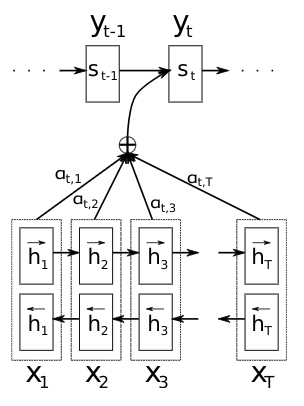
\includegraphics[width=180pt]{figure/ch01/rnndecoder.png}
  \caption{ภาพแสดงการทำงานของ Decoder ที่พัฒนาขึ้น ณ ขณะสร้างคำลำดับที่ t}
  \label{}
\end{figure}

เราใช้ feedforward neural network สำหรับคำนวณค่า alignment model นี้ ซึ่งทั้งหมดจะถูกฝึกสอนไปพร้อมๆ กับส่วนอื่นๆ ของระบบ  ซึ่งในส่วนของ alignment model นี้จะคำนวณแบบ soft alignment กล่าวคือ เราไม่ได้ระบุ alignment ที่ชัดเจนเหมือกับระบบแปลภาษาเชิงสถิติ แต่อาศัยน้ำหนักที่กำหนดสัดส่วนของบริบทในฝั่งอินพุต ซึ่งวิธีการนี้ทำให้ค่า gradient จาก cost function สามารถอัพเดตกลับมาที่พารามิเตอร์ของทั้งโครงข่ายได้โดยตลอด ซึ่งทำให้การอัพเดตพารามิเตอร์ทำได้ทั้งส่วนของ alignment และการแปลไปพร้อมๆ กัน

เราสามารถเข้าใจว่าการนำเอา annotation มาหาค่าเฉลี่ยถ่วงน้ำหนักนี้คือการหา expected annotation ซึ่งเป็นการหาค่าความคาดหวังของ alignment ที่เป็นไปได้ทั้งหมด เมื่อกำหนดให้ \myeq{ \alpha_{ij} }คือความน่าจะเป้นที่คำแปล \myeq{ y_i } จะสัมพันธ์กับคำในประโยคอินพุต \myeq{x_j} ดังนั้น context vector \myeq{c_i} ก็คือ ค่าความคาดหวังของ annotation (อาจเทียบได้กับบริบท) ของ annotation ทั้งหมดที่มี \myeq{a_{ij}} เป็นค่าความน่าจะเป็นที่ใช้คำนวณ

ค่าน้ำหนัก (ซึ่งมองเป็นความน่าจะเป็นได้) \myeq{a_{ij}}หรือ\myeq{e_{ij}} (ค่าพลังงานความเชื่อมโยง) นั้นสะท้อนให้เห็นถึงความสัมพันธ์ระหว่าง annotation\myeq{h_j} กับ hidden state ก่อนหน้า \myeq{s_{i-1}} เพื่อใช้ตัดสินใจเลือกคำแปลและคำนวณค่า hidden state ถัดไป วิธีการคำนวณใน decoder เช่นนี้เปรียบได้กับการสร้างระบบที่สามารถโฟกัสเฉพาะบางส่วนให้กับ decoder (เรียกว่า attention) ซึ่ง decoder เลือกส่วนของอินพุตที่ต้องการโฟกัส จากนั้นจึงแปลคำที่สัมพันธ์กับส่วนที่โฟกัสนั้นออกมา การสร้างระบบที่มีวิธีการนี้ช่วยลดภาระของ encoder ที่ต้องนำเอาข้อมูลทั้งหมดมาบีบอัดลงในเวกเตอร์เพียงตัวเดียว วิธีการเช่นนี้ทำให้ข้อมูลสามารถกระจายไปอยู่ในทุกๆ ส่วนของ encoder และตัว decoder จะทำหน้าที่เลือกส่วนของ encoder (annotation) มาแปลตามลำดับที่คำนวณได้จากขั้นตอน attention

\subsection{Encoder: Bidirectional RNN for Annotating Sequences}

RNN ที่ใช้ใน NMT แบบปกตินั้น (ดู Eq.1) จะอ่านอินพุต \myeq{x} โดยเริ่มจากคำแรก \myeq{x_1} ไปจนถึงสุดท้าย \myeq{ x_{\scaleto{T_x}{5pt}}} แต่ตามที่เราต้องการนำเสนอ เราไม่ต้องการให้ annotation นั้นมีข้อมูลเฉพาะคำก่อนหน้า แต่เรายังอยากให้มีข้อมูลของคำที่ตามหลังมาด้วย ดังนั้นเราจึงใช้ bidirectional RNN (BiRNN, Schuster and Paliwal, 1997) ซึ่งได้ผลดีกับงานทางด้าน speech recognition (ดู  Graves et al., 2013)


\end{document}